\section{10. Diagrama de Activity On Node}
\label{sec:AoN}

En la figura \ref{fig:AoN} se ilustra el diagrama de \textit{Activity on Node}. Las tareas están agrupadas en la misma forma que en la sección anterior:

\begin{enumerate}
\item Gestión del proyecto.
\item Investigación y capacitación en la arquitectura del microprocesador.
\item Desarrollo del ambiente de automatización.
\item Internalización de código pre-existente.
\item Investigación y capacitación en el framework de LLVM.
\item Desarrollo del software.
\item Desarrollo de tests unitarios y de API.
\item Documentación.
\item Presentación del trabajo.
\end{enumerate}

Cada tarea está etiquetada con una letra \textbf{T} seguida de su número de tarea. Por ejemplo, T1.1 corresponde a la tarea ``1.1 - Definición de requerimientos con el cliente''. El camino crítico, cuya duración es de 382 horas, se muestra resaltado en color rojo. El camino semicrítico se muestra resaltado en color azul. Mientras que el no crítico en se denota con una flecha puntuada.

\begin{figure}[htpb]
  \centering
  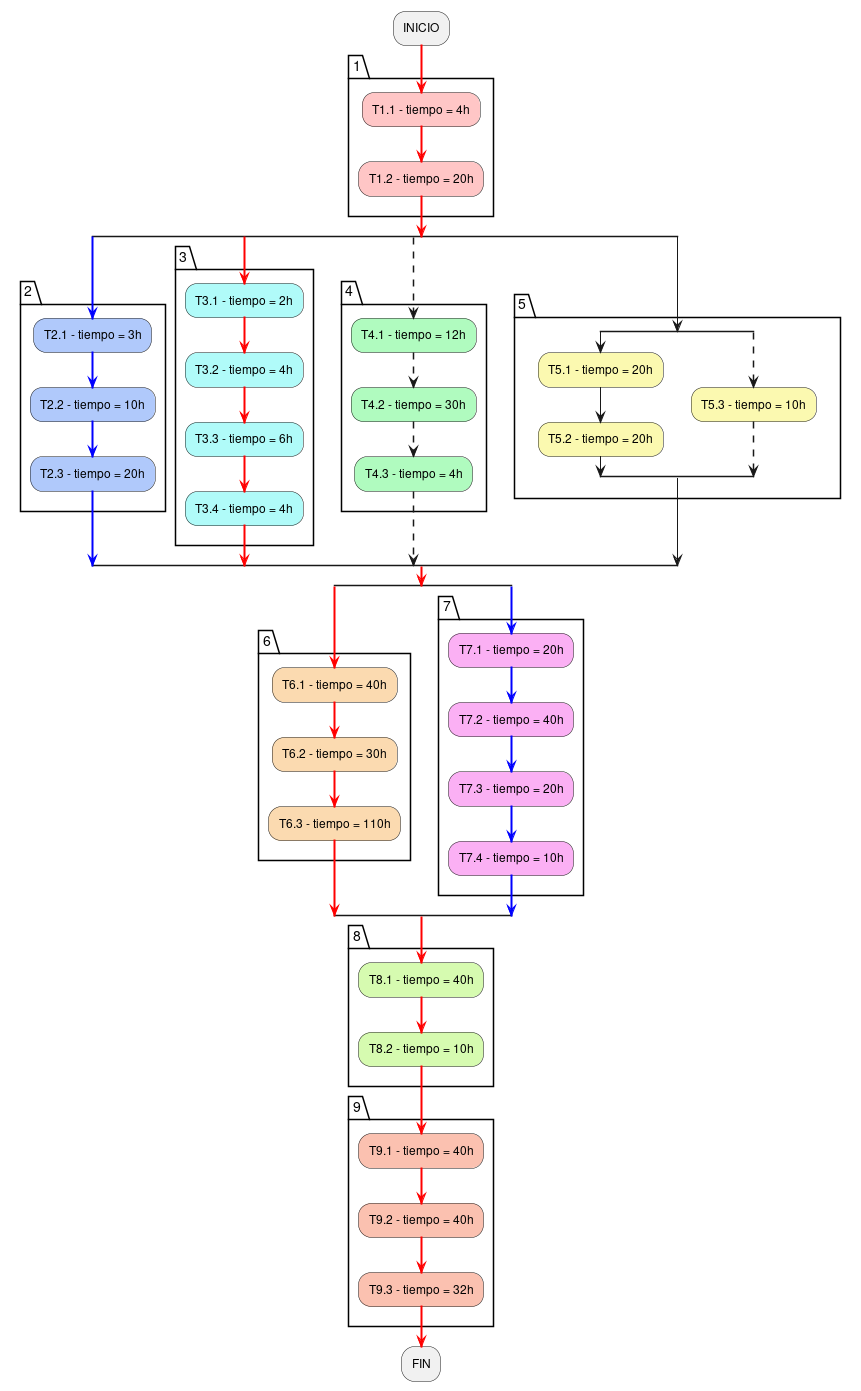
\includegraphics[width=.90\textwidth]{./assets/AoN.png}
  \caption{Diagrama de \textit{Activity on Node}.}
  \label{fig:AoN}
\end{figure}

\vspace{25px}
